\documentclass[12pt,a4paper]{article}

% ─── Page Layout ───────────────────────────────────────────────────────────────
\usepackage[a4paper, margin=0.8in, headheight=14pt]{geometry}

% ─── Fonts (XeLaTeX) ───────────────────────────────────────────────────────────
\usepackage{fontspec}
\usepackage{unicode-math}
\setmainfont{TeX Gyre Pagella}
\setmonofont[Scale=0.88]{TeX Gyre Cursor}
\setmathfont{Latin Modern Math}

% ─── Packages ──────────────────────────────────────────────────────────────────
\usepackage{xcolor}
\usepackage{colortbl}
\usepackage{titlesec}
\usepackage{enumitem}
\usepackage{tabularx}
\usepackage{booktabs}
\usepackage{array}
\usepackage{amsmath}
\usepackage{tikz}
\usetikzlibrary{shapes.geometric, arrows.meta, positioning, calc, fit, decorations.pathreplacing}
\usepackage{tcolorbox}
\tcbuselibrary{skins, breakable}
\usepackage{hyperref}
\usepackage{fancyhdr}
\usepackage{graphicx}
\usepackage{microtype}
\hyphenpenalty=10000
\exhyphenpenalty=10000
\sloppy
\usepackage{caption}
\usepackage{setspace}
\usepackage{multirow}
\usepackage{tocloft}

% ─── Q&A helper ────────────────────────────────────────────────────────────────
\newcommand{\Q}[1]{\textbf{#1}\par\noindent\ignorespaces}

% ─── Colour Palette ────────────────────────────────────────────────────────────
\definecolor{myred}{RGB}{196,30,58}
\definecolor{mydark}{RGB}{30,30,50}
\definecolor{mygreen}{RGB}{14,120,80}
\definecolor{myteal}{RGB}{0,130,140}
\definecolor{myamber}{RGB}{180,100,0}
\definecolor{mypurple}{RGB}{100,30,160}
\definecolor{mygray}{RGB}{246,247,249}
\definecolor{mgframe}{RGB}{180,185,200}
\definecolor{watermark}{RGB}{145,150,170}
\definecolor{hdrred}{RGB}{250,232,235}
\definecolor{hdrgreen}{RGB}{220,244,233}
\definecolor{hdrteal}{RGB}{220,242,244}
\definecolor{hdramber}{RGB}{253,242,215}
\definecolor{hdrpurple}{RGB}{238,228,255}
\definecolor{hdrgray}{RGB}{238,240,245}
\definecolor{rowalt}{RGB}{250,251,253}

% ─── Section Formatting ────────────────────────────────────────────────────────
\titleformat{\section}
  {\large\bfseries\color{myred}}{\thesection.}{0.5em}{}
  [\vspace{1pt}{\color{myred}\rule{\linewidth}{0.8pt}}]
\titleformat{\subsection}
  {\normalsize\bfseries\color{myteal}}{\thesubsection}{0.5em}{}
\titlespacing*{\section}{0pt}{18pt}{7pt}
\titlespacing*{\subsection}{0pt}{11pt}{4pt}

% ─── Paragraph ─────────────────────────────────────────────────────────────────
\setlength{\parindent}{0pt}
\setlength{\parskip}{4pt}

% ─── TOC Styling ───────────────────────────────────────────────────────────────
\renewcommand{\cfttoctitlefont}{\large\bfseries\color{myred}}
\renewcommand{\cftaftertoctitle}{\par\noindent{\color{myred}\rule{\linewidth}{0.8pt}}}
\setlength{\cftbeforetoctitleskip}{0pt}
\setlength{\cftaftertoctitleskip}{6pt}
\renewcommand{\cftsecfont}{\normalsize\bfseries\color{mydark}}
\renewcommand{\cftsecpagefont}{\normalsize\bfseries\color{mydark}}
\renewcommand{\cftsecleader}{\cftdotfill{\cftdotsep}}
\setlength{\cftbeforesecskip}{7pt}
\renewcommand{\cftsubsecfont}{\small\color{mydark}}
\renewcommand{\cftsubsecpagefont}{\small\color{mydark}}
\setlength{\cftbeforesubsecskip}{3pt}
\setlength{\cftsubsecindent}{1.4em}

% ─── Table helpers ─────────────────────────────────────────────────────────────
\renewcommand{\arraystretch}{1.45}
\setlength{\tabcolsep}{6pt}
\arrayrulecolor{mydark}
\newcolumntype{B}[1]{>{\small\bfseries\raggedright\arraybackslash}m{#1}}
\newcolumntype{Y}{>{\small\raggedright\arraybackslash}X}
\renewcommand{\tabularxcolumn}[1]{m{#1}}

% ─── Header / Footer ───────────────────────────────────────────────────────────
\pagestyle{fancy}
\fancyhf{}
\fancyhead[L]{\small\color{myred}\textbf{HS-HU701}\;\color{mydark}--- Principles of Management}
\fancyhead[R]{\small\color{myteal}\textbf{Module 3 Notes}}
\fancyfoot[C]{\small\color{mydark}\thepage}
\fancyfoot[R]{\small\color{watermark}\textit{\copyright\ Biraj}}
\renewcommand{\headrulewidth}{0.5pt}
\renewcommand{\footrulewidth}{0.3pt}

% ─── Hyperref ──────────────────────────────────────────────────────────────────
\hypersetup{
  colorlinks=true, linkcolor=myteal, urlcolor=myteal,
  pdfauthor={Biraj Sarkar},
  pdftitle={HS-HU701 --- Module 3 Notes}
}

% ─── tcolorbox styles ──────────────────────────────────────────────────────────
\tcbset{
  tikzbox/.style={
    colback=mygray, colframe=mgframe, boxrule=0.6pt, arc=4pt,
    left=8pt, right=8pt, top=6pt, bottom=6pt,
    colbacktitle=mgframe, coltitle=mydark,
    fonttitle=\small\bfseries
  },
  defbox/.style={
    colback=hdrgreen, colframe=mygreen, boxrule=0.8pt, arc=4pt,
    left=9pt, right=9pt, top=6pt, bottom=6pt,
    colbacktitle=mygreen, coltitle=white,
    fonttitle=\small\bfseries
  },
  formulabox/.style={
    colback=hdrteal, colframe=myteal, boxrule=0.8pt, arc=4pt,
    left=9pt, right=9pt, top=7pt, bottom=7pt,
    colbacktitle=myteal, coltitle=white,
    fonttitle=\small\bfseries
  },
  examplebox/.style={
    colback=hdramber, colframe=myamber, boxrule=0.8pt, arc=4pt,
    left=9pt, right=9pt, top=6pt, bottom=6pt,
    colbacktitle=myamber, coltitle=white,
    fonttitle=\small\bfseries
  },
  masonbox/.style={
    colback=hdrpurple, colframe=mypurple, boxrule=0.8pt, arc=4pt,
    left=9pt, right=9pt, top=6pt, bottom=6pt,
    colbacktitle=mypurple, coltitle=white,
    fonttitle=\small\bfseries
  },
  exambox/.style={
    colback=hdrpurple, colframe=mypurple, boxrule=1pt, arc=5pt,
    left=10pt, right=10pt, top=8pt, bottom=8pt,
    colbacktitle=mypurple, coltitle=white,
    fonttitle=\bfseries,
    breakable, title after break={\textbf{Frequently Asked / Viva Questions (contd.)}}}
}
\tcbset{breakable}

% ─── TikZ styles ───────────────────────────────────────────────────────────────
\tikzset{
  block/.style={rectangle, draw=myteal, fill=hdrteal,
    text width=2.4cm, align=center, minimum height=0.95cm,
    font=\small, rounded corners=3pt, line width=0.7pt},
  redblock/.style={rectangle, draw=myred, fill=hdrred,
    text width=2.4cm, align=center, minimum height=0.95cm,
    font=\small, rounded corners=3pt, line width=0.7pt},
  netnode/.style={rectangle, draw=myteal, fill=hdrteal,
    text width=1.5cm, align=center, minimum height=0.8cm,
    font=\small, rounded corners=3pt, line width=0.7pt},
  sumjunc/.style={circle, draw=myamber, fill=hdramber,
    minimum size=0.62cm, font=\small, line width=0.8pt},
  snode/.style={circle, draw=mypurple, fill=hdrpurple,
    minimum size=0.55cm, font=\footnotesize, line width=0.7pt},
  arrow/.style={-Stealth, thick, color=mydark},
  redarrow/.style={-Stealth, thick, color=myred},
  line/.style={thick, color=mydark}
}

% ═══════════════════════════════════════════════════════════════════════════════
\begin{document}
% ═══════════════════════════════════════════════════════════════════════════════

\begin{center}
  {\LARGE\bfseries\color{myred} HS-HU701 --- Principles of Management}\\[5pt]
  {\normalsize\color{mydark} Semester VII \quad$\bullet$\quad 2L:0T:0P \quad$\bullet$\quad 2 Credits}\\[3pt]
  {\normalsize\color{myteal}\textbf{Module 3 Exam Notes}}\\[3pt]
  {\small\color{mydark} CGEC \;$|$\; B.Tech ECE (2023--27) \;$|$\; \textit{Biraj Sarkar}}
\end{center}
\vspace{2pt}
\noindent{\color{myred}\rule{\linewidth}{1.5pt}}
\vspace{2pt}

\hypersetup{linkcolor=mydark}
\tableofcontents
\hypersetup{linkcolor=myteal}
\newpage

% ===============================================================================
\section{Leadership}
% ===============================================================================

\begin{tcolorbox}[defbox, title={\textbf{Leadership --- Definition}}]
\textbf{Leadership} is the ability to influence, inspire, and guide others toward the achievement of organisational goals. A leader motivates followers to willingly exert effort toward common objectives.
\par\vspace{3pt}
\textbf{Manager vs.\ Leader:} A manager is appointed (formal authority); a leader may be formal or informal. Managers administer; leaders innovate. Managers maintain; leaders develop.
\end{tcolorbox}

\subsection{Concept and Nature of Leadership}
\begin{itemize}[leftmargin=*, itemsep=3pt]
  \item Leadership is a process, not just a position or trait.
  \item It involves a triad: \textbf{leader}, \textbf{followers}, and \textbf{situational context}.
  \item Effective leaders adapt their style to the readiness and needs of followers.
  \item Leadership is forward-looking; it involves creating a vision and aligning people toward it.
\end{itemize}

\subsection{Leadership Styles}

\par\noindent
\begin{tabularx}{\linewidth}{|B{3.0cm}|Y|Y|}
\hline
\rowcolor{hdrgray}
\multicolumn{1}{|>{\centering\arraybackslash}m{3.0cm}|}{\textbf{Style}} &
\multicolumn{1}{>{\centering\arraybackslash}Y|}{\textbf{Description}} &
\multicolumn{1}{>{\centering\arraybackslash}Y|}{\textbf{Best Suited For}} \\
\hline
Autocratic & Leader makes all decisions alone; high control, low participation. & Crises, unskilled workers, urgent tasks. \\
\hline
Democratic / Participative & Leader involves team in decision-making; shares authority. & Skilled/experienced teams; creative tasks. \\
\hline
Laissez-Faire / Free-Rein & Leader delegates fully; minimal intervention. & Highly skilled experts; research teams. \\
\hline
Transformational & Leader inspires change through vision, charisma, and individual attention. & Organisational change; long-term innovation. \\
\hline
Transactional & Leader motivates through reward and punishment; maintains the status quo. & Routine, well-defined tasks. \\
\hline
Servant Leadership & Leader prioritises the needs of followers; facilitates growth and well-being. & Service-oriented organisations, NGOs. \\
\hline
\end{tabularx}

\subsection{Key Leadership Theories}

\subsubsection{Trait Theory}
Leadership is determined by inherent personal qualities --- physical, mental, and personality characteristics. Key traits identified: intelligence, self-confidence, integrity, decisiveness, drive, and sociability.
\par\vspace{3pt}
\textbf{Limitation:} Does not explain why people with the same traits succeed in some situations and fail in others.

\subsubsection{Behavioural Theories}
Focus on what leaders \textit{do} rather than what they \textit{are}:
\begin{itemize}[leftmargin=*, itemsep=2pt]
  \item \textbf{Ohio State Studies:} Two dimensions --- \textbf{Initiating Structure} (task-oriented) and \textbf{Consideration} (people-oriented). Best leaders are high on both.
  \item \textbf{Michigan Studies:} \textbf{Production-centred} vs.\ \textbf{Employee-centred} leadership. Employee-centred leaders achieve higher productivity and satisfaction.
  \item \textbf{Blake--Mouton Managerial Grid:} Plots leadership on two axes --- concern for production (1--9) and concern for people (1--9). Ideal is (9,9) = Team Management.
\end{itemize}

\begin{tcolorbox}[tikzbox, title={Blake--Mouton Managerial Grid}]
\centering
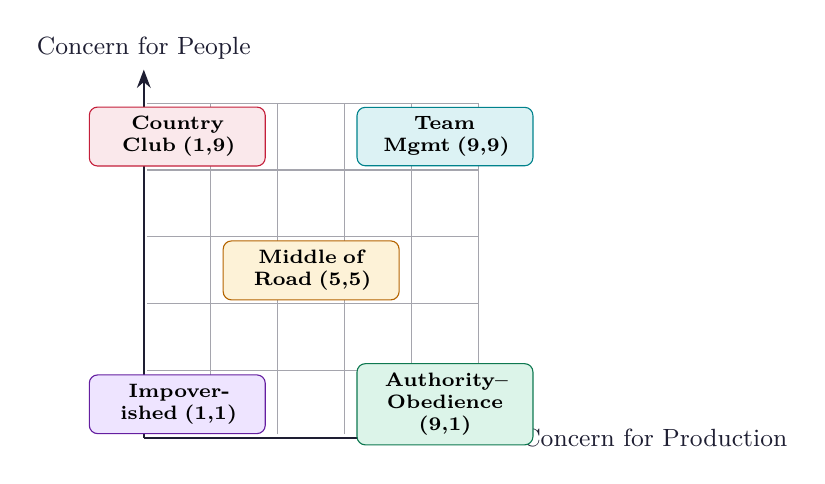
\begin{tikzpicture}[scale=0.85]
  \draw[-Stealth, thick, color=mydark] (0,0) -- (5.5,0) node[right, font=\small] {Concern for Production};
  \draw[-Stealth, thick, color=mydark] (0,0) -- (0,5.5) node[above, font=\small] {Concern for People};

  \foreach \x in {1,2,3,4,5} \draw[color=mydark!40, thin] (\x,0.05)--(\x,5);
  \foreach \y in {1,2,3,4,5} \draw[color=mydark!40, thin] (0.05,\y)--(5,\y);

  \node[draw=myred, fill=hdrred, rounded corners=3pt, font=\scriptsize\bfseries,
    text width=2.0cm, align=center, minimum height=0.65cm] at (0.5,4.5) {Country Club (1,9)};
  \node[draw=myteal, fill=hdrteal, rounded corners=3pt, font=\scriptsize\bfseries,
    text width=2.0cm, align=center, minimum height=0.65cm] at (4.5,4.5) {Team Mgmt (9,9)};
  \node[draw=myamber, fill=hdramber, rounded corners=3pt, font=\scriptsize\bfseries,
    text width=2.0cm, align=center, minimum height=0.65cm] at (2.5,2.5) {Middle of Road (5,5)};
  \node[draw=mypurple, fill=hdrpurple, rounded corners=3pt, font=\scriptsize\bfseries,
    text width=2.0cm, align=center, minimum height=0.65cm] at (0.5,0.5) {Impoverished (1,1)};
  \node[draw=mygreen, fill=hdrgreen, rounded corners=3pt, font=\scriptsize\bfseries,
    text width=2.0cm, align=center, minimum height=0.65cm] at (4.5,0.5) {Authority--Obedience (9,1)};
\end{tikzpicture}
\end{tcolorbox}

\subsubsection{Situational/Contingency Theories}
Leadership effectiveness depends on the match between the leader's style and the situation:
\begin{itemize}[leftmargin=*, itemsep=2pt]
  \item \textbf{Fiedler's Contingency Model:} Leadership effectiveness depends on the match between the leader's style (task vs.\ relationship oriented) and situational favourableness (leader--member relations, task structure, position power).
  \item \textbf{Hersey--Blanchard Situational Leadership:} Leader adapts style (Telling $\to$ Selling $\to$ Participating $\to$ Delegating) based on follower \textit{readiness} (competence + commitment).
  \item \textbf{Path--Goal Theory (House):} Leader's job is to remove obstacles and provide guidance (directive, supportive, participative, achievement-oriented) to help followers reach their goals.
\end{itemize}

% ===============================================================================
\section{Decision Making}
% ===============================================================================

\begin{tcolorbox}[defbox, title={\textbf{Decision Making --- Definition}}]
\textbf{Decision Making} is the process of identifying and selecting a course of action to solve a specific problem or capitalise on an opportunity. It is the core of managerial activity and involves choosing among alternatives under conditions of certainty, risk, or uncertainty.
\end{tcolorbox}

\subsection{Concept and Nature of Decision Making}
\begin{itemize}[leftmargin=*, itemsep=3pt]
  \item \textbf{Pervasive:} Decision making occurs at all levels and in all functions of management.
  \item \textbf{Continuous:} Managers make decisions constantly throughout their working day.
  \item \textbf{Goal-Directed:} Every decision is aimed at solving a problem or achieving an objective.
  \item \textbf{Selection Among Alternatives:} Decision making implies the existence of two or more possible choices.
\end{itemize}

\subsection{Types of Decisions}
\par\noindent
\begin{tabularx}{\linewidth}{|B{3.2cm}|Y|Y|}
\hline
\rowcolor{hdrgray}
\multicolumn{1}{|>{\centering\arraybackslash}m{3.2cm}|}{\textbf{Type}} &
\multicolumn{1}{>{\centering\arraybackslash}Y|}{\textbf{Description}} &
\multicolumn{1}{>{\centering\arraybackslash}Y|}{\textbf{Example}} \\
\hline
Programmed (Structured) & Routine, repetitive decisions handled by standard procedures and rules. & Processing a standard purchase order. \\
\hline
Non-Programmed (Unstructured) & Novel, complex, non-routine decisions requiring judgment. & Entering a new international market. \\
\hline
Strategic & Long-term, top-level decisions affecting the entire organisation. & Mergers and acquisitions. \\
\hline
Tactical & Medium-term decisions by middle management to implement strategy. & Annual budget allocation. \\
\hline
Operational & Short-term, day-to-day decisions at the operational level. & Employee shift scheduling. \\
\hline
\end{tabularx}

\subsection{The Decision-Making Process}

\begin{tcolorbox}[tikzbox, title={Rational Decision-Making Process}]
\centering
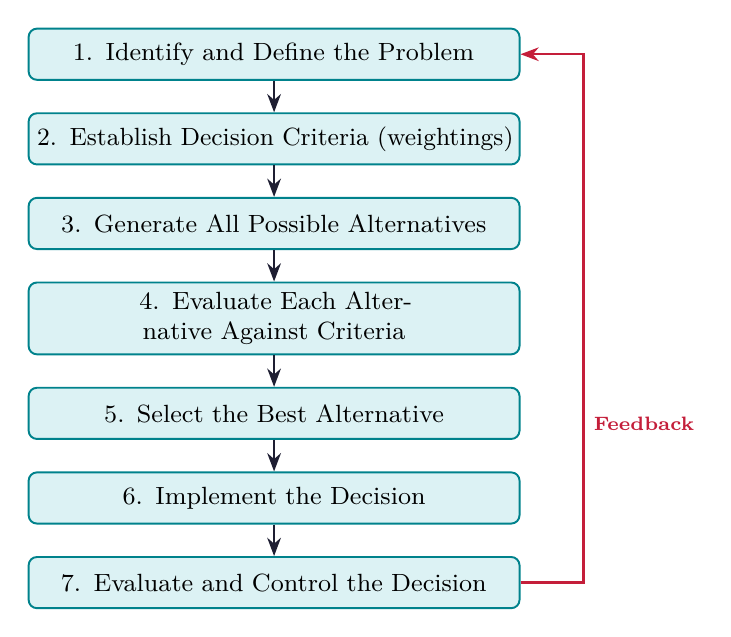
\begin{tikzpicture}[
  stepbox/.style={rectangle, draw=myteal, fill=hdrteal, text width=6.0cm,
    align=center, minimum height=0.65cm, font=\small, rounded corners=3pt, line width=0.7pt},
  arrow/.style={-Stealth, thick, color=mydark}
]
  \node[stepbox] (s1) {1. Identify and Define the Problem};
  \node[stepbox, below=0.4cm of s1] (s2) {2. Establish Decision Criteria (weightings)};
  \node[stepbox, below=0.4cm of s2] (s3) {3. Generate All Possible Alternatives};
  \node[stepbox, below=0.4cm of s3] (s4) {4. Evaluate Each Alternative Against Criteria};
  \node[stepbox, below=0.4cm of s4] (s5) {5. Select the Best Alternative};
  \node[stepbox, below=0.4cm of s5] (s6) {6. Implement the Decision};
  \node[stepbox, below=0.4cm of s6] (s7) {7. Evaluate and Control the Decision};

  \draw[arrow] (s1)--(s2); \draw[arrow] (s2)--(s3); \draw[arrow] (s3)--(s4);
  \draw[arrow] (s4)--(s5); \draw[arrow] (s5)--(s6); \draw[arrow] (s6)--(s7);
  \draw[redarrow] (s7.east) -- ++(0.8,0) |- (s1.east)
    node[pos=0.15, right, font=\scriptsize\bfseries\color{myred}] {Feedback};
\end{tikzpicture}
\end{tcolorbox}

\subsection{Decision-Making Tools and Techniques}

\begin{itemize}[leftmargin=*, itemsep=3pt]
  \item \textbf{Brainstorming:} Group technique for generating maximum creative alternatives without criticism.
  \item \textbf{Delphi Technique:} Structured consensus-building among experts through successive anonymous questionnaires.
  \item \textbf{Decision Tree:} A graphical tool showing a sequence of decisions and their possible outcomes, payoffs, and probabilities.
  \item \textbf{Pay-off Matrix:} A table showing payoffs for each decision under each state of nature; used under uncertainty.
  \item \textbf{Cost--Benefit Analysis (CBA):} Compares the total expected costs and benefits of alternatives; choose the alternative with the highest net benefit.
  \item \textbf{Linear Programming (LP):} Optimises an objective function (maximise profit, minimise cost) subject to linear constraints.
  \item \textbf{SWOT Analysis:} Evaluates Strengths, Weaknesses, Opportunities, and Threats to guide strategic decisions.
\end{itemize}

% ===============================================================================
\section{Economic, Financial and Quantitative Analysis}
% ===============================================================================

\subsection{Production and Markets}

\begin{tcolorbox}[defbox, title={\textbf{Production and Market Structures}}]
\textbf{Production} is the process of transforming inputs (labour, capital, raw materials) into outputs (goods and services). Market structure defines the competitive environment in which firms operate.
\end{tcolorbox}

\par\noindent
\begin{tabularx}{\linewidth}{|B{2.8cm}|Y|Y|Y|}
\hline
\rowcolor{hdrgray}
\multicolumn{1}{|>{\centering\arraybackslash}m{2.8cm}|}{\textbf{Structure}} &
\multicolumn{1}{>{\centering\arraybackslash}Y|}{\textbf{Sellers}} &
\multicolumn{1}{>{\centering\arraybackslash}Y|}{\textbf{Price Control}} &
\multicolumn{1}{>{\centering\arraybackslash}Y|}{\textbf{Example}} \\
\hline
Perfect Competition & Many & None (price takers) & Agricultural markets. \\
\hline
Monopolistic Competition & Many & Some (product differentiation) & Restaurants, clothing. \\
\hline
Oligopoly & Few & Significant & Telecom, automobile. \\
\hline
Monopoly & One & Full (price maker) & Utility companies. \\
\hline
\end{tabularx}

\subsection{National Income Accounting}

\begin{tcolorbox}[formulabox, title={\textbf{National Income Concepts}}]
\renewcommand{\arraystretch}{1.3}
\begin{tabularx}{\linewidth}{B{4.5cm} X}
GDP (Expenditure) & $\text{GDP} = C + I + G + (X - M)$ \\[4pt]
NNP at Market Price & $\text{NNP}_{MP} = \text{GNP}_{MP} - \text{Depreciation}$ \\[4pt]
National Income (NI) & $\text{NI} = \text{NNP}_{MP} - \text{Indirect Taxes} + \text{Subsidies}$ \\[4pt]
Personal Income & $\text{PI} = \text{NI} - \text{Retained Earnings} - \text{Corp.\ Taxes} + \text{Transfer Payments}$ \\[4pt]
Disposable Income & $\text{DI} = \text{PI} - \text{Personal Taxes}$
\end{tabularx}
\par\vspace{4pt}
Where: $C$ = Consumption, $I$ = Investment, $G$ = Government spending, $X - M$ = Net exports.
\end{tcolorbox}

\subsection{Financial Function and Goals}

\begin{tcolorbox}[defbox, title={\textbf{Financial Management \& Functions}}]
\textbf{Financial Management} deals with the procurement and efficient utilisation of funds to achieve the goals of an enterprise. 

The three core \textbf{Financial Functions} (decision-making areas) are:
\begin{enumerate}[leftmargin=*, itemsep=2pt, topsep=2pt]
  \item \textbf{Investment Decisions (Capital Budgeting):} Allocation of capital to long-term assets to generate future returns.
  \item \textbf{Financing Decisions (Capital Structure):} Choosing the best mix of debt and equity to minimise the overall cost of capital.
  \item \textbf{Dividend Decisions:} Deciding the proportion of net profits to distribute as dividends versus retaining them for reinvestment.
\end{enumerate}
\end{tcolorbox}

\textbf{Goals of Financial Management:}\par\noindent
The primary objective of financial management is guiding capital decisions. The two major approaches are:
\begin{itemize}[leftmargin=*, itemsep=2pt]
  \item \textbf{Profit Maximisation:} Focuses on increasing net profits or earnings per share (EPS).
  \item \textbf{Wealth Maximisation (Shareholder Value Maximisation):} Focuses on increasing the net present value (NPV) of the firm's equity, reflected in the market value of its shares.
\end{itemize}

\par\noindent
\begin{tabularx}{\linewidth}{|B{3.0cm}|Y|Y|}
\hline
\rowcolor{hdrgray}
\multicolumn{1}{|>{\centering\arraybackslash}m{3.0cm}|}{\textbf{Aspect}} &
\multicolumn{1}{>{\centering\arraybackslash}Y|}{\textbf{Profit Maximisation}} &
\multicolumn{1}{>{\centering\arraybackslash}Y|}{\textbf{Wealth Maximisation}} \\
\hline
Primary Goal & Maximize accounting profits. & Maximize market price of shares (NPV of firm). \\
\hline
Time Value of Money & Ignores the timing of cash inflows. & Considers the timing of cash inflows (discounting). \\
\hline
Risk and Uncertainty & Ignores risk associated with future earnings. & Directly accounts for risk and uncertainty. \\
\hline
Focus & Short-term performance. & Long-term sustainable growth and value. \\
\hline
Limitation & Vague definition of ``profit'' (gross, net, pre-tax). & Requires efficient financial markets to reflect true value. \\
\hline
\end{tabularx}

\subsection{Financial Statement Analysis}

\begin{tcolorbox}[defbox, title={\textbf{Financial Statements}}]
\textbf{Balance Sheet:} Snapshot of financial position at a point in time (Assets = Liabilities + Equity).
\par\vspace{3pt}
\textbf{Income Statement (P\&L):} Shows revenues, expenses, and profit/loss over a period.
\par\vspace{3pt}
\textbf{Cash Flow Statement:} Tracks actual cash inflows and outflows from operations, investing, and financing activities.
\end{tcolorbox}

\textbf{Key Financial Ratios:}\par\noindent
\begin{tabularx}{\linewidth}{|B{3.2cm}|Y|Y|}
\hline
\rowcolor{myteal}
\multicolumn{1}{|>{\centering\arraybackslash\color{white}}m{3.2cm}|}{\textbf{Category}} &
\multicolumn{1}{>{\centering\arraybackslash\color{white}}Y|}{\textbf{Ratio}} &
\multicolumn{1}{>{\centering\arraybackslash\color{white}}Y|}{\textbf{Formula}} \\
\hline
Liquidity & Current Ratio & Current Assets / Current Liabilities \\
\hline
Liquidity & Quick Ratio & (Current Assets $-$ Inventory) / Current Liabilities \\
\hline
Profitability & Net Profit Margin & Net Profit / Net Sales $\times$ 100 \\
\hline
Profitability & Return on Equity (ROE) & Net Profit / Shareholders' Equity $\times$ 100 \\
\hline
Leverage & Debt-to-Equity & Total Debt / Shareholders' Equity \\
\hline
Activity & Inventory Turnover & Cost of Goods Sold / Average Inventory \\
\hline
\end{tabularx}

\subsection{Quantitative Methods --- Statistical Inference}

\begin{tcolorbox}[defbox, title={\textbf{Statistical Inference}}]
\textbf{Statistical Inference} is the process of drawing conclusions about population parameters based on data from a sample. Key concepts: hypothesis testing, confidence intervals, and significance levels.
\end{tcolorbox}

\begin{tcolorbox}[formulabox, title={\textbf{Hypothesis Testing --- Z-test for Population Mean}}]
\renewcommand{\arraystretch}{1.3}
\begin{tabularx}{\linewidth}{B{4.0cm} X}
Test Statistic & $\displaystyle z = \frac{\bar{x} - \mu_0}{\sigma / \sqrt{n}}$ \\[8pt]
Standard Error & $\displaystyle SE = \frac{\sigma}{\sqrt{n}}$ \\[8pt]
Confidence Interval & $\displaystyle \mu \in \left(\bar{x} - z_{\alpha/2} \cdot SE,\;\; \bar{x} + z_{\alpha/2} \cdot SE\right)$
\end{tabularx}
\par\vspace{4pt}
Reject $H_0$ if $|z| > z_{\alpha/2}$ (two-tailed test). Common: $z_{0.025} = 1.96$ for 95\% confidence.
\end{tcolorbox}

\subsection{Forecasting}

\begin{tcolorbox}[defbox, title={\textbf{Forecasting}}]
\textbf{Forecasting} is the process of using historical data, trends, and judgments to predict future values (demand, sales, costs). It reduces uncertainty in planning and decision-making.
\end{tcolorbox}

\textbf{Common forecasting methods:}
\begin{itemize}[leftmargin=*, itemsep=2pt]
  \item \textbf{Moving Average:} Average of the most recent $n$ data points; smooths out fluctuations.
  \item \textbf{Exponential Smoothing:} Weighted moving average where more recent data receives greater weight.
  \item \textbf{Trend Projection:} Fits a least-squares regression line to historical data and projects it forward.
  \item \textbf{Qualitative methods:} Delphi, market surveys, jury of executive opinion --- used when historical data is absent.
\end{itemize}

\begin{tcolorbox}[formulabox, title={\textbf{Simple Linear Regression (Trend Line)}}]
\renewcommand{\arraystretch}{1.3}
\begin{tabularx}{\linewidth}{B{4.0cm} X}
Regression Line & $\hat{y} = a + bx$ \\[4pt]
Slope & $\displaystyle b = \frac{n\sum xy - \sum x \sum y}{n \sum x^2 - \left(\sum x\right)^2}$ \\[8pt]
Intercept & $\displaystyle a = \frac{\sum y - b\sum x}{n}$ \\[6pt]
Correlation Coefficient & $\displaystyle r = \frac{n\sum xy - \sum x \sum y}{\sqrt{[n\sum x^2 - (\sum x)^2][n\sum y^2 - (\sum y)^2]}}$
\end{tabularx}
\par\vspace{4pt}
$|r| = 1$: perfect correlation; $r = 0$: no linear correlation. $r^2$ (coefficient of determination) measures the proportion of variance explained.
\end{tcolorbox}

\subsection{Statistical Quality Control (SQC)}

\begin{tcolorbox}[defbox, title={\textbf{Statistical Quality Control (SQC)}}]
\textbf{SQC} is the application of statistical methods to monitor and control a production process so that the process operates at its full potential and produces conforming products.
\end{tcolorbox}

\textbf{Key tools of SQC:}
\begin{itemize}[leftmargin=*, itemsep=3pt]
  \item \textbf{Control Charts:} Monitor process variation over time. Central Line (CL), Upper Control Limit (UCL), and Lower Control Limit (LCL) are plotted. Common types: $\bar{X}$-chart (mean), R-chart (range), p-chart (proportion defective).
  \item \textbf{Acceptance Sampling:} Inspecting a random sample from a batch; accept or reject the entire batch based on the sample result.
  \item \textbf{Process Capability Index ($C_p$, $C_{pk}$):} Measures how well a process meets specifications.
\end{itemize}

\begin{tcolorbox}[formulabox, title={\textbf{Control Chart Limits for \texorpdfstring{$\bar{X}$}{X-bar} Chart}}]
\renewcommand{\arraystretch}{1.3}
\begin{tabularx}{\linewidth}{B{3.5cm} X}
Centre Line (CL) & $\bar{\bar{X}}$ (grand mean of all subgroup means) \\[4pt]
Upper Control Limit & $\text{UCL} = \bar{\bar{X}} + A_2 \bar{R}$ \\[4pt]
Lower Control Limit & $\text{LCL} = \bar{\bar{X}} - A_2 \bar{R}$
\end{tabularx}
\par\vspace{4pt}
$A_2$ = tabulated constant based on subgroup size $n$; $\bar{R}$ = average range.
A point outside UCL or LCL signals an \textbf{out-of-control} (assignable cause) condition.
\end{tcolorbox}

% ===============================================================================
% MANDATORY QUICK REVISION PAGE
% ===============================================================================
\newpage
\begin{center}
  {\large\bfseries\color{myred} Quick Revision --- Module 3}\\[3pt]
  {\small\color{mydark} Leadership, Decision Making \& Quantitative Analysis $|$ HS-HU701}
\end{center}
\noindent{\color{myred}\rule{\linewidth}{1.2pt}}
\vspace{4pt}

\begin{tcolorbox}[formulabox, title={\textbf{Key Formulas at a Glance}}]
\renewcommand{\arraystretch}{1.3}
\begin{tabularx}{\linewidth}{B{4.2cm} X}
GDP (Expenditure) & $C + I + G + (X - M)$ \\[3pt]
National Income & $\text{GNP}_{MP} - \text{Depreciation} - \text{Indirect Taxes} + \text{Subsidies}$ \\[3pt]
Z-test Statistic & $z = (\bar{x} - \mu_0) / (\sigma / \sqrt{n})$ \\[3pt]
Regression Slope & $b = (n\sum xy - \sum x \sum y) / (n\sum x^2 - (\sum x)^2)$ \\[3pt]
X-bar UCL / LCL & $\bar{\bar{X}} \pm A_2 \bar{R}$ \\[3pt]
Current Ratio & Current Assets / Current Liabilities \\[3pt]
Net Profit Margin & Net Profit / Net Sales $\times 100$ \\
\end{tabularx}
\end{tcolorbox}

\begin{tcolorbox}[defbox, title={\textbf{One-Line Definitions}}]
\begin{itemize}[leftmargin=*, itemsep=2pt, topsep=0pt]
  \item \textbf{Leadership:} Ability to influence and guide others toward achieving goals.
  \item \textbf{Autocratic Leadership:} Leader makes all decisions unilaterally with full authority.
  \item \textbf{Transformational Leadership:} Inspires change through vision, charisma, and motivation.
  \item \textbf{Decision Making:} Process of selecting a course of action from available alternatives.
  \item \textbf{Programmed Decision:} Routine decision resolved by standard procedures.
  \item \textbf{Non-Programmed Decision:} Novel, complex decision requiring managerial judgment.
  \item \textbf{GDP:} Total monetary value of all goods and services produced within a country in a year.
  \item \textbf{SQC:} Use of statistical methods to monitor and control production quality.
  \item \textbf{Control Chart:} Graphical tool to detect process variation over time using UCL and LCL.
  \item \textbf{Regression Analysis:} Statistical method to model the relationship between variables.
  \item \textbf{Forecasting:} Using historical data and trends to predict future values.
\end{itemize}
\end{tcolorbox}

\begin{tcolorbox}[exambox, title={\textbf{Frequently Asked / Viva Questions}}]
\begin{enumerate}[topsep=0pt, label=\textbf{Q\arabic*.}, itemsep=5pt]
  \item \Q{What is leadership? How does a leader differ from a manager?}
    Leadership is the ability to influence others toward goals. A manager has formal authority (appointed), while a leader may be informal. Managers administer; leaders innovate. Leaders inspire; managers control.
  \item \Q{Name and explain the three basic leadership styles.}
    Autocratic (leader decides alone), Democratic (team participates in decisions), Laissez-Faire (leader delegates fully with minimal intervention).
  \item \Q{What is the Blake--Mouton Managerial Grid? What is the ideal position?}
    A grid plotting concern for production (x-axis) vs.\ concern for people (y-axis), each on a 1--9 scale. The ideal position is (9,9) Team Management --- high concern for both people and production.
  \item \Q{What is Hersey--Blanchard Situational Leadership theory?}
    Leaders adapt their style (Telling $\to$ Selling $\to$ Participating $\to$ Delegating) based on the follower's readiness level (combination of competence and commitment).
  \item \Q{Distinguish between programmed and non-programmed decisions.}
    Programmed decisions are routine and repetitive, handled by standard rules (e.g., stock reorder). Non-programmed decisions are novel and complex, requiring judgment (e.g., entering a new market).
  \item \Q{What is the Decision Tree technique?}
    A graphical representation of a decision problem showing decision nodes (squares), chance nodes (circles), possible outcomes, and associated probabilities and payoffs, enabling rational selection of the best path.
  \item \Q{What is GDP? Write its expenditure-side formula.}
    GDP (Gross Domestic Product) is the total monetary value of all final goods and services produced within a country in a year. Expenditure formula: $\text{GDP} = C + I + G + (X - M)$.
  \item \Q{What is Statistical Quality Control (SQC)? Name its key tools.}
    SQC is the use of statistical methods to monitor and control production processes. Key tools: Control Charts ($\bar{X}$-chart, R-chart, p-chart), Acceptance Sampling, and Process Capability Indices.
  \item \Q{What do UCL and LCL represent in a control chart?}
    UCL (Upper Control Limit) and LCL (Lower Control Limit) are the boundaries of natural process variation (set at $\pm 3\sigma$). A plotted point outside these limits indicates an out-of-control (assignable cause) condition.
  \item \Q{State the formula for simple linear regression.}
    $\hat{y} = a + bx$, where $b$ is the slope and $a$ is the intercept. The slope is $b = (n\sum xy - \sum x \sum y) / (n\sum x^2 - (\sum x)^2)$.
  \item \Q{What is the purpose of financial ratio analysis?}
    It allows comparison of a firm's performance against its own historical data, competitors, or industry benchmarks. Key categories: liquidity (current ratio), profitability (ROE), leverage (debt-to-equity), and activity (inventory turnover).
  \item \Q{What is the difference between Transformational and Transactional leadership?}
    Transformational leaders inspire change through vision and motivation (long-term focus). Transactional leaders use reward--punishment to maintain performance within existing norms (short-term, routine focus).
\end{enumerate}
\end{tcolorbox}

\begin{tcolorbox}[tikzbox, title={Types of Decisions --- Comparison Table}]
\centering
\renewcommand{\arraystretch}{1.4}
\begin{tabularx}{\linewidth}{|B{3.0cm}|Y|Y|}
\hline
\rowcolor{hdrgray}
\multicolumn{1}{|>{\centering\arraybackslash}m{3.0cm}|}{\textbf{Aspect}} &
\multicolumn{1}{>{\centering\arraybackslash}Y|}{\textbf{Programmed Decision}} &
\multicolumn{1}{>{\centering\arraybackslash}Y|}{\textbf{Non-Programmed Decision}} \\
\hline
Nature & Routine, repetitive & Novel, unique \\
\hline
Level & Lower/Middle management & Top management \\
\hline
Time & Short-term & Long-term \\
\hline
Basis & Standard rules, procedures & Judgment, creativity \\
\hline
Risk & Low & High \\
\hline
Example & Payroll processing & Product launch strategy \\
\hline
\end{tabularx}
\end{tcolorbox}

\end{document}
